\chapter{Analysis}
This chapter will go through the the analyzing process of specifying and narrowing down, more specific requirements from the overall requirements established at the start of the project.  Additionally, it will also discuss the fundamental changes that were made to the requirements and why it that was the case

\section{Use Cases}
An overall requirement list, such as the aforementioned, is a good beginning to establish the core features and requirements the system needed to have in order to have a working product. However it is not enough to more accurately describe the exact requirements needed in order to develop such a system from the ground up.  In order to establish these requirements a more precise requirement list is needed to be found. 

Firstly the primary requirements, consisting of requirements mandatory to the systems overall functionality, is rooted out. These requirements is then analyzed through the creation of Use Cases. These use cases represents a user going through a part of a system. This is also called the flow of events. An example of such a Use Case is shown here below. All of the Use Cases created for this project is in the Appendix, Figure A.6 to A.12
\begin{figure}[ht]
    \centering
    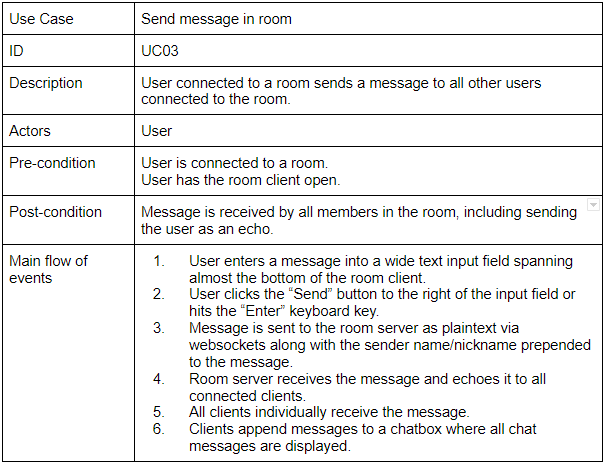
\includegraphics[width=\textwidth]{Pictures/UseCaseSendMessage.png}
    \caption{Use Case for when a user inputs a message to the group it is connected to.}
    \label{fig:gantt}
\end{figure}

Establishing these use cases for the primary parts of the system gives a more specific and described insight as to what requirements is missing, needs adjusting or is excessive. Through this process a more descriptive requirement specification is created. 

\section{Finalized Requirement Specification}
This table below illustrates the different requirements established from the analysis above. In addition, a general MoSCoW prioritization is performed, to indicate what requirements is the most important to implement. This is illustrated in the "MoSCoW" column. The "Use Case" column shows how the the different requirements fit the Use Cases that the requirements is derived from. The "Evaluation" column indicates how each requirement is tested and evaluated. 

The requirements is structured as main requirements that describe the use case its derived from and sub-requirements that go into detail. The verification column point to a specific subsection of the Verification chapter, where information about the verification of the requirement is available.

\begin{table}[h]
\begin{tabularx}{\textwidth}{|l|X|l|l|l|}
\hline
ID  & Description & MosCoW & Use Case & Verification \\ \hline\hline
\textbf{R01} & Rooms is composed of a Kubernetes deployment. & M & & \ref{vR01} \\ \hline
R01.1 & Room pods must be able to send and receive live packages (socket server). & M & & \ref{vR01.1}       \\ \hline
R01.2 & Room pods must be automatically created on demand. & M & & \ref{vR01.2}         \\ \hline
\textbf{R02} & Individual users is consisting of a served website & M & & \ref{vR02}      \\ \hline
R02.1 & Webserver must be scalable using Kubernetes & M & & \ref{vR02.1}      \\ \hline
\textbf{R03} & Connect to rooms & M & UC01 & \ref{vR03}      \\ \hline
R03.1 & Rooms each have a unique URL with its ID. & S & & \ref{vR03.1}     \\ \hline
R03.2 & RoomFinder service uses room ID to retrieve unique room pod URL from database & M & & \ref{vR03.2}      \\ \hline
R03.3 & Database containing room information & M & & \ref{vR03.3}      \\ \hline
R03.4 & Joining room requires entering of a nickname & S & & \ref{vR03.4}      \\ \hline
\end{tabularx}
\caption{Part 1/2 of the finished requirement specification}
\label{tab:risks}
\end{table}

\begin{table}[htb]
\begin{tabularx}{\textwidth}{|l|X|l|l|l|}
\hline
R04 & Send message in rooms & M & UC03 & \ref{vR04}    \\ \hline
R04.1 & Messages sent to room pod socket server & M & & \ref{vR04.1}    \\ \hline
R04.2 & Users connected to room pod socket server receives messages & M & & \ref{vR04.2}    \\ \hline
R05 & Create rooms & M & UC08 & \ref{vR05}    \\ \hline
R05.1 & Creates room with unique ID & M & & \ref{vR05.1}   \\ \hline
R06 & User movement & S & UC04 & \ref{vR06}    \\ \hline
R06.1 & User can click on area on screen and move to that point & C & & \ref{vR06.1}   \\ \hline
R06.2 & User position updates and sent to other users in group periodically & S & & \ref{vR06.2}    \\ \hline
R06.3 & Other users positions is updated to represent user movement & S & & \ref{vR06.3}     \\ \hline
R06.4 & Movement updates voice stream service with new position. & S & & \ref{vR06.4}    \\ \hline
R07 & Video and voice connection. & S & UC07 & \ref{vR07}     \\ \hline
R07.1 & WebRTC connection & S & & \ref{vR07.1}   \\ \hline
R07.1.1 & Signalling server as a Kubernetes pod & S & & \ref{vR07.1.1}    \\ \hline
\end{tabularx}
\caption{Part 2/2 of the finished requirement specification}
\label{tab:risks}
\end{table}

\newpage
\section{Changes to requirements after implementation iterations}
The above requirements is the foundation and guidance of which the design and implementation takes from in order to establish a fully fledged system of the same vision that was originally envisioned. However when going through these phases, it becomes more apparent which requirements might not be viable, is not necessary or is blatantly wrong. These are deemed not viable, either due to ignorance around the would-be-used technologies at the time, not necessary due to design changes made in the design phase or implementation phase, or having the prioritizing change due to time constraints.

\section{Selected Technologies}

In order to implemented the requirements elicited from the analysis of initial requirements, a set of technologies and tools have been chosen to facilitate the system. These technologies are outlined here, as well as how they are used in the project.

\subsection{Kubernetes}

Kubernetes is an open-source platform for managing containerized deployments, services or workloads. The main difference between traditional deployments and containerized deployments is that a container is its own virtualized environment, which makes the deployment of said containers simple across many different platforms. With Kubernetes it is possible to automatically scale these containerized services, in the case of an increase in traffic, expose the services, so that it is accessible to users on the internet, and load balance the network traffic to ensure the system is stable. \cite{kubernetes}

This project can use Kubernetes to expose and load balance the network traffic to the system. Additionally, core containers make use of Kubernetes workload management, and will create more containers if the system requires. 

\subsection{Node.js}

In contrast to normal Javascript, which is mostly used for client-side functionality, Node JS is a Javascript runtime environment, primarily used for back-end development such as web servers and API’s. Node JS uses an event-driven architecture, which makes Node JS great at handling the many output and input operations a web-server receives.\cite{nodejs}

Node JS can be used extensively in this project, to implement the components in a quick and easy manner, in addition to handling the website for the clients. Node JS applications are also easy to establish tests for, with a myriad of different packages providing tools for testing.

\subsection{Socket.io}

Socket.io is a way to communicate real time with the server on the browser. Socket.io sets up a Websocket connection between the browser and the server, which is used to transport the messages to and from both ends quickly and reliably. \cite{socketio} 

This project can use Socket.io to facilitate connections between different clients of the system, in order to give clients the ability to communicate with each other. Additionally, it can be used to keep track of clients' positions and make sure that position was updated on every other client's applications. WebSockets are a strong alternative contender, but it is felt that the additional features provided by socket.io, such as rooms, could come in use.

\subsection{WebRTC}

WebRTC, short for Web Real Time Communication, is a framework that makes it possible to set up real-time communication pipelines between users directly, instead of going through a web-server. This is called peer-to-peer communication.  WebRTC can be used to communicate with audio, video or basic data streams. In order to create these peer-to-peer connections, the users must first negotiate and discover each other. This is done in a process called signalling. Using a web-server, the users are sending each other information about themselves, in order to be able to connect. If successful, a WebRTC connection is established. \cite{webrtc}

WebRTC is an excellent candidate for a communications framework used to enable audio and video communication, as indicated by its frequent use in competing products. This has been implemented in two different ways in this project. The standard peer-to-peer connection and a Media Relay Server (MRS). 

\subsection{GitHub Actions}

GitHub Actions is a newer CI/CD framework compared to alternatives such as Travis CI. However, GitHub Actions is a particular favored framework due to it's great accessibility, and ease of use. Naturally, it is also about as integrated into GitHub, the version control service that this project has made use of, as possible. GitHub Actions function similarly to other CI/CD frameworks by having developers write some sort of YAML file which contains instructions on what actions the CI/CD pipeline must perform, such as a Docker Build or Publish action.\cite{githubactionsdocs}

This project can make use of GitHub Actions to automate unit and integration tests of system components, and have the tests execute each time a change is pushed to the GitHub repositories.

\section{Conclusion}
Going from the overall requirements determined during the projects inception, to a specified requirements list is an important process in order to specify what requirements are necessary in order to move on to the design phase. Using these requirements it was possible to keep track on what was required to take into account during the design phase, needed to implement during the implementation phase, and important aspects to evaluate during the evaluation phase. A number of specific tools and technologies such as perhaps most notably Node.js, Socket.io, and WebRTC, are strong contenders for use in creating the system.